\documentclass{standalone}

\usepackage{libertine}
\usepackage[libertine]{newtxmath}
\usepackage{relsize}

\usepackage[dvipsnames]{xcolor}
\usepackage[outline]{contour}

\usepackage{tikz}
\usetikzlibrary{calc, arrows.meta}

\usepackage{macros}


\begin{document}
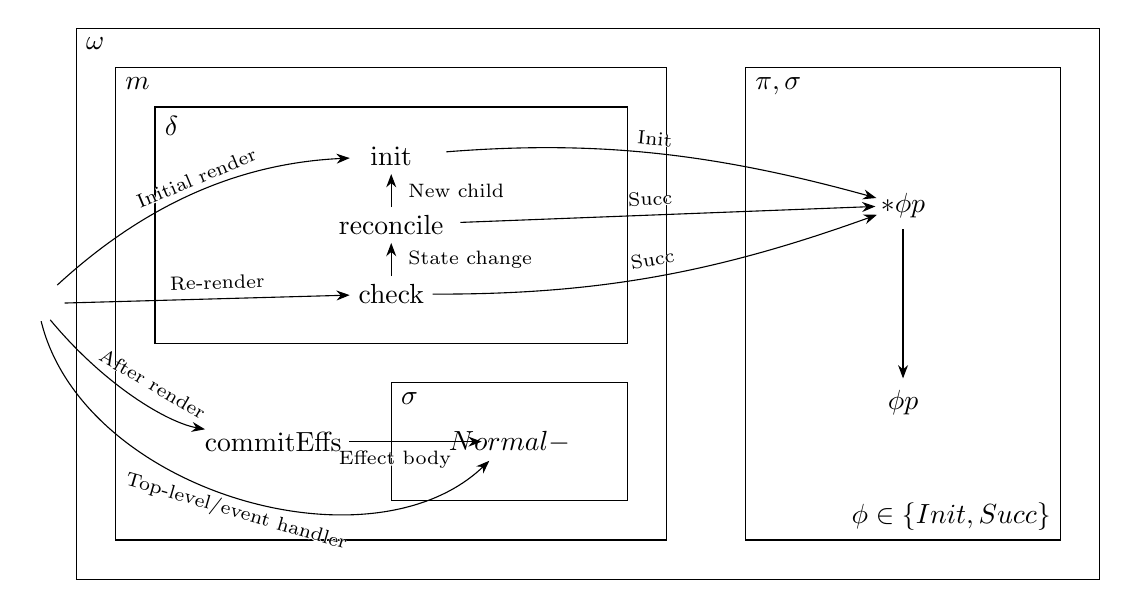
\begin{tikzpicture}[>=Stealth]
  \coordinate (bl) at (0, 0);
  \coordinate (br) at (13, 0);
  \coordinate (tl) at (0, 6);
  \coordinate (tr) at (13, 6);
  \coordinate (wbl) at (0.5, -0.5);
  \coordinate [label=-45:$\omega$]
              (wtl) at (0.5, 6.5);
  \coordinate (wtr) at (13.5, 6.5);
  \coordinate (mbl) at (1, 0);
  \coordinate (mbr) at (8, 0);
  \coordinate [label=-45:$m$]
              (mtl) at (1, 6);
  \coordinate (mtr) at (8, 6);
  \coordinate (dbl) at (1.5, 2.5);
  \coordinate (dbr) at (7.5, 2.5);
  \coordinate [label=-45:$\delta$]
              (dtl) at (1.5, 5.5);
  \coordinate (dtr) at (7.5, 5.5);
  \coordinate (pbl) at (9, 0);
  \coordinate [label=135:{$\phi \in \{\phase{Init}, \phase{Succ}\}$}]
              (pbr) at (13, 0);
  \coordinate [label=-45:{$\pi, \sigma$}]
              (ptl) at (9, 6);
  \coordinate (ptr) at (13, 6);
  \coordinate (sbl) at (4.5, 0.5);
  \coordinate (sbr) at (7.5, 0.5);
  \coordinate [label=-45:$\sigma$]
              (stl) at (4.5, 2);
  \coordinate (str) at (7.5, 2);

  % \draw [help lines] (bl) grid (tr);

  \draw  (wbl) rectangle (wtr);
  \draw  (mbl) rectangle (mtr)
                         (dbl) rectangle (dtr)
                         (pbl) rectangle (ptr)
                         (sbl) rectangle (str);

  \coordinate (smallstep) at ($(bl)!0.5!(tl)$);
  \coordinate (evalnorm) at ($(sbl)!0.5!(str)$);
  \coordinate (commitEffs) at ($(evalnorm) - (3, 0)$);
  \coordinate (reconcile) at ($(dbl)!0.5!(dtr)$);
  \coordinate (check) at ($(reconcile) - (0, 0.875)$);
  \coordinate (render) at ($(reconcile) + (0, 0.875)$);
  \coordinate (evalmult) at ($(pbl)!0.5!(ptr) + (0, 1.25)$);
  \coordinate (eval) at ($(pbl)!0.5!(ptr) - (0, 1.25)$);

  \node at (smallstep) {$\smallstep$};
  \node at (evalnorm) {$\Bigstep{\mathrlap{\phase{Normal}}}{\mathrlap{-}}$};
  \node at (commitEffs) {\sem{commitEffs}};
  \node at (reconcile) {\sem{reconcile}};
  \node at (check) {\sem{check}};
  \node at (render) {\sem{init}};
  \node at (evalmult) {$\Bigstep*{\mathrlap{\phi}}{\mathrlap{p}}$};
  \node at (eval) {$\Bigstep{\mathrlap{\phi}}{\mathrlap{p}}$};

  \draw [->, shorten <=1em, shorten >=1.5em] (smallstep) to [bend left=20] node [sloped, above] {\smaller[2] \contour{white}{Initial render}} (render);
  \draw [->, shorten <=1em, shorten >=1.5em] (smallstep) to node [sloped, above] {\smaller[2] Re-render} (check);

  \draw [->, shorten <=1.5ex, shorten >=1.5ex] (check) to node [right] {\smaller[2] State change} (reconcile);
  \draw [->, shorten <=1.5ex, shorten >=1.5ex] (reconcile) to node [right] {\smaller[2] New child} (render);

  \draw [->, shorten <=2em, shorten >=1em] (render) to [bend left=10] node [sloped, above] {\smaller[2] \contour{white}{\phase{Init}}} (evalmult);
  \draw [->, shorten <=2.5em, shorten >=1em] (reconcile) to node [sloped, above] {\smaller[2] \contour{white}{\phase{Succ}}} (evalmult);
  \draw [->, shorten <=1.5em, shorten >=1em] (check) to [bend right=10] node [sloped, above] {\smaller[2] \contour{white}{\phase{Succ}}} (evalmult);

  \draw [->, shorten <=2ex, shorten >=2ex] (evalmult) to (eval);

  \draw [->, shorten <=1.75ex, shorten >=2.5em] (smallstep) to [bend right=20] node [sloped, above] {\smaller[2] \contour{white}{After render}} (commitEffs);
  \draw [->, shorten <=2.75em, shorten >=1em] (commitEffs) to node [below] {\smaller[2] \contour{white}{Effect body}} (evalnorm);
  \draw [->, shorten <=1.5ex, shorten >=1em] (smallstep) to [bend right=60] node [sloped, below] {\smaller[2] \contour{white}{Top-level/event handler}} (evalnorm);
\end{tikzpicture}
\end{document}
